\section{Envisioned final product}
An early concept of the final product can be found in figure \ref{fig:e-reader}.
The device will have a tablet design with multiple rows of letters that would allow the user to read through text in a manner similar to reading through a page.
The multiple rows also allow for the development of extra features in the future, such as scientific use(e.g. Graph Representation).
The device will most likely utilize magnetic elastic actuators for the control and the pins.The electromagnets will be controlled using an Arduino Micro-controller.
However, due to the time limitation of this project and possible modifications during the development process, the prototype produced may vary to the envisioned product (e.g. Less number of rows, bulkier casing).
Finally, that's only an original concept and is subject to being revisited.

\begin{figure}[h]
\centering
    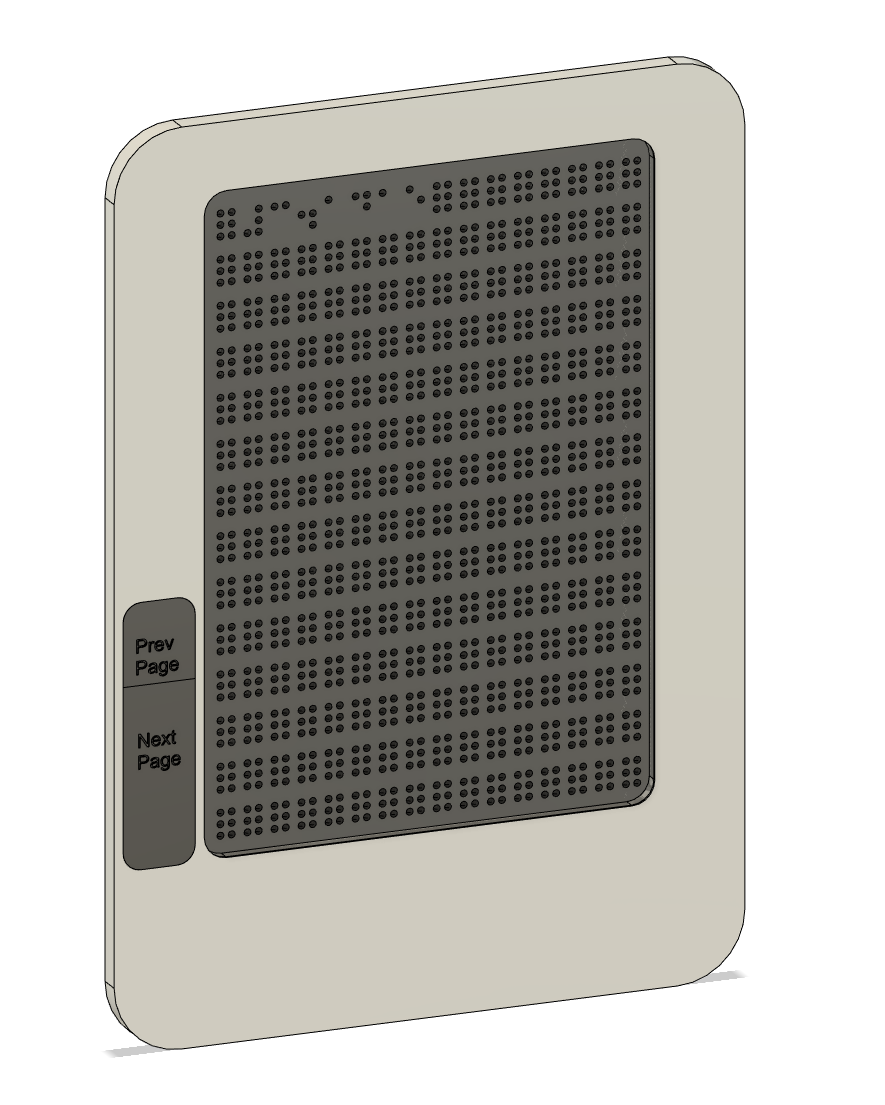
\includegraphics[width=0.4\textwidth]{figures/e-reader.png}
\caption[Envisioned finished product]{Envisioned finished product. A Braille version of a standard e-reader aimed to provide broadened access and display information a traditional Braille device can't.}
\label{fig:e-reader}
\end{figure}

% \subsection{Encoding}
% Figure \ref{fig:encoding.png} describes the initial approach to convert text into braille given a device with 16 addressable cells.
% \begin{figure}
% \centering
%     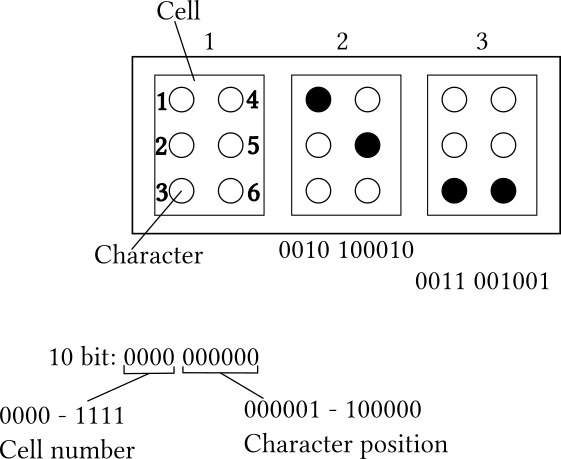
\includegraphics[height=5cm]{figures/encoding.png}
% \caption{Early idea for serial encoding of up to 16 braille cells.}
% \label{fig:encoding.png}
% \end{figure}

\section{Actuator technology}
    \subsection{Addressable cell}
        \subimport{technologies/}{addressable-cell.tex}
    \subsection{Individually addressable characters}
        \subsubsection{Piezoelectric}
        \subimport{technologies/}{piezoelectric.tex}
        
        \subsubsection{Pneumatic}
        \subimport{technologies/}{pneumatic.tex}

        \subsubsection{Magnetic}
        \subimport{technologies/}{magnetic.tex}

        \subsubsection{Others}
        \subimport{technologies/}{others.tex}